\chapter{Progettazione Logica}
\section{Stima del volume dei dati}
Segue una tabella riportante una stima del numero di Record che popoleranno il Database finale. Molte Entità risultano avere un volume molto compatto e preciso.\newline
È importante notare che il numero di persone presenti del Database potrebbe influenzare pesantemente le due Entità principali, "Tabella degli Aspetti" e "Tabella dei Placement". Per semplicità ipotizziamo di inserire un migliaio di persone all'interno del sistema.
{\rowcolors{2}{black!20!white!50}{black!10!white!50}
\begin{longtable}{ |p{4cm}|p{6cm}|  }
%\hline
\endfoot
\hline
\textbf{ENTITÀ} & \textbf{VOLUME STIMATO (RECORD)} \\
\hline
Aspetto & \begin{math} \simeq 5 \end{math} \\
Casa Astrologica & \begin{math} \equiv 5 \end{math} \\
Citta & \begin{math} \simeq 48000 \end{math} \\
Domicili & \begin{math} \equiv 16 \end{math} \\
Elemento & \begin{math} \equiv 4 \end{math}\\
Modo & \begin{math} \equiv 3 \end{math} \\
Persona & Molto variabile, \begin{math} \simeq 1000 \end{math} \\
Punto del Cielo & \begin{math} \geq 13 \end{math} \\
Regione & \begin{math} \simeq 4500 \end{math} \\
Segno Zodiacale & \begin{math} \equiv 12 \end{math} \\
Stato & \begin{math} \simeq 300 \end{math} \\
Tabella degli Aspetti & \begin{math} (39 \cdot |Persona|) \Rightarrow \quad \simeq 39000 \end{math} \\
Tabella dei Placement & \begin{math} (7 \cdot |Persona|) \Rightarrow \quad \simeq 7000 \end{math} \\
\hline
\end{longtable}
}
I valori 39 e 7 delle ultime due Entità non sono casuali.\newline
Il coefficiente binomiale \begin{math} \binom{13}{2} \end{math} corrisponde al numero di coppie di punti possibili, se ci sono 13 punti. Facendo una semplice media, ricaviamo che una persona mediamente ha circa 39 aspetti. In realtà la densità degli aspetti è molto difficile da approssimare. Calcolare un valore accurato è pressochè impossibile, per cui 39 è un valore abbastanza accettabile.\newline
Lo stesso ragionamento vale per i Placement, ogni persona può avere al massimo 13 Placement se ci sono 13 punti, quindi mediamente una persona ne ha circa 7.
\textbf{Osservazione:} Il numero di aspetti nella "Tabella degli aspetti" dipende ANCHE dal numero di Tuple in "Aspetti", per semplificare sono stati usati solo il numero di Persone e il numero dei Punti.
I valori di Stato, Regione e Citta sono stati arrotondati a valori multipli di 10. Le tabelle finali usate nel Database per queste tre entità sono state reperite su internet, e sono completamente open source.
\section{Descrizione delle operazioni principali}
\label{sec:opprinc}
Le operazioni principali richieste sono le seguenti:
\begin{enumerate}
	\item Aggiunta e rimozione di una persona dal sistema.
	\item Aggiunta e rimozione del Placement di una persona.
	\item Aggiunta e rimozione degli Aspetti di una persona.
	\item Visualizzazione di tutte le informazioni astrologiche di una persona.
	\item Ricavare se possibile, dettagli astrologici della persona, per esempio:
	\begin{itemize}
		\item Ricavare il pianeta di domicilio del segno solare di una persona.
		\item Ricavare quali pianeti sono in domicilio tra i Placement di una persona.
	  \item Ricavare il numero di modi/elementi di ciascuno segno posseduto da una persona.
		\item Ricavare la casa più popolata di una persona.
		\item Ricavare la firma zodiacale di una persona.\textbf{*}
	\end{itemize}
\end{enumerate}
\textbf{*}: La firma zodiacale è il segno zodiacale che ha il modo e l'elemento che appaiono di piú tra i pianeti di una persona.
\section{Frequenza delle Operazioni}
La seguente tabella riporta per ogni operazione sopra elencata una stima della loro frequenza.
{\rowcolors{2}{black!20!white!50}{black!10!white!50}
\begin{longtable}{ |p{10cm}|p{3cm}|  }
%\hline
\endfoot
\hline
\textbf{Operazione} & \textbf{Frequenza} \\
\hline
Aggiunta di una persona & 10/Settimana\\
Rimozione di una persona & 1/Mese \\
Aggiunta di un placement & 600/Settimana \\
Rimozione di un placement & 20/Settimana \\
Aggiunta di un aspetto & 1000/Settimana \\
Rimozione di un aspetto & 50/Settimana \\
Visualizzazione di tutte le info astrologiche di una persona & 20/Settimana \\
Visualizzazione dei dettagli astrologici (tutti) & 20/Settimana \\
\hline
\end{longtable}
}

\section{Tabelle degli Accessi}
Ora che possediamo sia una stima del volume dei dati sia una stima della frequenza delle operazioni principali, possiamo valutare i costi di ogni operazione. Il costo di una singola lettura vale 1, mentre quello di una scrittura vale doppio. Verrà usato come riferimento lo schema logico anzichè il concettuale, in riferimento alla figura \ref{fig:finalschemelogic}.
{\rowcolors{2}{black!20!white!50}{black!10!white!50}
\begin{longtable}{ |p{3cm}|p{4cm}|p{4.5cm}|}
%\hline
\endfoot
\hline
\textbf{Operazione} & \textbf{Concetti} & \textbf{Costo (al Mese)} \\
\hline
Aggiunta di una persona & Persona & (1S) * 40 = \textbf{80}\\
Rimozione di una persona & Persona,\newline TabellaDeiPlacement,\newline TabellaDegliAspetti  & ((1S) + (7S) + (39S)) = \textbf{94} \\
Aggiunta di un Placement & TabellaDeiPlacement & (1S) * 2400 = \textbf{4800}\\
Rimozione di un Placement & TabellaDeiPlacement & (1S) * 80 = \textbf{160}\\
Aggiunta di un Aspetto & TabellaDegliAspetti & (1S) * 4000 = \textbf{8000}\\
Rimozione di un Aspetto & TabellaDegliAspetti & (1S) * 200 = \textbf{400}\\
Visualizzazione di tutte le info astrologiche di una persona (nel caso peggiore) & Persona,\newline TabellaDegliAspetti,\newline TabellaDeiPlacement,\newline PuntoDelCielo,\newline CasaAstrologica,\newline SegnoZodiacale,\newline Aspetto &
((1L) + (7L) + (39L) + (7L) + (7L) + (7L) + (5L)) * 80 = \textbf{5840}\\
Pianeti di Domicilio del segno solare & PuntoDelCielo,\newline Domicilio,\newline SegnoZodiacale & ((1L) + (2L) + (2L)) * 80 = \textbf{400}\\
Pianeti in Domicilio & PuntoDelCielo,\newline Domicilio,\newline SegnoZodiacale & ((7L) + (14L) + (14L)) * 80 = \textbf{2800}\\
Numero degli Elementi di una Persona & TabellaDeiPlacement,\newline SegnoZodiacale & (7L) + ((7L) * 4) * 80 = \textbf{2800}\\
Numero dei Modi di una Persona & TabellaDeiPlacement,\newline SegnoZodiacale & (7L) + ((7L) * 3) * 80 = \textbf{2240}\\
Casa piú popolata di una Persona & TabellaDeiPlacement,\newline SegnoZodiacale & (7L) * 80= \textbf{560}\\
\hline
Firma Zodiacale di una Persona & SegnoZodiacale,\newline Modo,\newline Elemento & ((7L) + (7L) + (1L)) * 80= \textbf{1200}\\
\hline
\end{longtable}
}

\section{Raffinamento dello schema concettuale}
Lo schema concettuale in figura \ref{fig:finalscheme} deve essere tradotto in uno schema Logico.\newline
\subsection{Rimozione di Attributi Composti}
L'unico attributo composto presente nello schema concettuale si trova nell'entità Persona.\newline
Per gestirlo nel migliore dei modi sono state usate tabelle open source reperite su internet. Compaiono quindi 3 nuove Enitità, Stato, Regione e Città. Sarà necessario memorizzare nella persona solo la città, la quale possiede un codice univoco. Grazie alle chiavi esterne si possono facilmente ricavare lo Stato e la Regione partendo dalla città.
\subsection{Rimozione della Gerarchia}
L'unica gerarchia presente nello schema riguarda i Punti del Cielo, ed è di tipo Totale/Esclusiva.\newline
Si è scelto di adottare come soluzione un collasso verso l'alto. Tutti i punti possiedono caratteristiche molto simili in termini pratici. Inoltre, risulta molto più comodo e veloce reperire informazione da un'unica Entità piuttosto che da tre.\newline
Unica nota, è necessario aggiungere un attributo "Tipo" all'Entità finale "Punto del Cielo" per distinguere la tipologia di ogni punto. Per comodità, anche l'attributo "Tipo" stesso è stato tradotto in un' Entità, il cui unico attributo è Tipo che rappresenta anche la Chiave Primaria.
\subsection{Chiavi Primarie e Chiavi Esterne}
Le chiavi primarie sono state già ben definite nello schema concettuale. Di seguito vengono comunque elencate le Entità e le corrispondenti Chiavi Primarie. Le chiavi esterne sono state inserite nelle entità corrispondenti, in base alle cardinalità dello schema concettuale (Figura \ref{fig:finalscheme}). Riportiamo nella seguente lista anche le chiavi esterne, e le rispettive rinominazioni:\newline\newline
\textbf{Stato}:\newline
\textbf{PK}: \underline{ID}\newline\newline
\textbf{Regione}:\newline
\textbf{PK}: \underline{ID}\newline
\textbf{FK}: ID importata dall'entità \textbf{Stato}, rinominata in \textit{ID\_Stato}\newline\newline
\textbf{Citta}:\newline
\textbf{PK}: \underline{ID}\newline
\textbf{FK}: ID importata dall'entità \textbf{Regione}, rinominata in \textit{ID\_Regione}\newline\newline
\textbf{Modo}:\newline
\textbf{PK}: \underline{Numero}\newline\newline
\textbf{Elemento}:\newline
\textbf{PK}: \underline{Numero}\newline\newline
\textbf{Segno Zodiacale}:\newline
\textbf{PK}: \underline{Numero}\newline
\textbf{FK}: Numero importata dall'entità \textbf{Modo}, rinominata in \textit{Modo}\newline
\textbf{FK}: Numero importata dall'entità \textbf{Elemento}, rinominata in \textit{Elemento}\newline\newline
\textbf{Casa Astrologica}:
\textbf{PK}: \underline{Governante}\newline
\textbf{FK}: Numero importata dall'entità \textbf{Segno Zodiacale}, rinominata in \textit{Governante}\newline\newline
\textbf{Aspetto}:\newline
\textbf{PK}: \underline{Angolo}\newline\newline
\textbf{Tipo Punto}:\newline
\textbf{PK}: \underline{Tipo}\newline\newline
\textbf{Punto Del Cielo}:
\textbf{PK}: \underline{Numero}\newline
\textbf{FK}: Tipo importata dall'entità \textbf{Tipo Punto}, non rinominata.\newline\newline
\textbf{Domicilio}:
\textbf{PK}: (\underline{Segno}, \underline{Punto})\newline
\textbf{FK}: Numero importata dall'entità \textbf{Segno}, rinominata in \textit{Segno}.\newline
\textbf{FK}: Numero importata dall'entità \textbf{Punto Del Cielo}, rinominata in \textit{Punto}.\newline\newline
\textbf{Persona}:\newline
\textbf{PK}: \underline{ID}\newline\newline
\textbf{Tabella Dei Placement}:\newline
\textbf{PK}: (\underline{IDPersona}, \underline{Punto})\newline
\textbf{FK}: ID importata dall'entità \textbf{Persona}, rinominata in \textit{IDPersona}.\newline
\textbf{FK}: Numero importata dall'entità \textbf{Punto Del Cielo}, rinominata in \textit{Punto}.\newline
\textbf{FK}: Numero importata dall'entità \textbf{Segno Zodiacale}, rinominata in \textit{Segno}.\newline
\textbf{FK}: Governante importata dall'entità \textbf{Casa Astrologica}, rinominata in \textit{Casa}.\newline\newline
\textbf{Tabella Degli Aspetti}:\newline
\textbf{PK}: (\underline{IDPersona}, \underline{PrimoPunto}, \underline{SecondoPunto})\newline
\textbf{FK}: ID importata dall'entità \textbf{Persona}, rinominata in \textit{IDPersona}.\newline
\textbf{FK}: Numero importata dall'entità \textbf{Punto Del Cielo}, rinominata in \textit{PrimoPunto}.\newline
\textbf{FK}: Numero importata dall'entità \textbf{Punto Del Cielo}, rinominata in \textit{SecondoPunto}.\newline
\section{Traduzione in modello relazionale}
Le entità vengono tradotte in modello relazionale, in un ordine tale da permettere l'importazione delle chiavi esterne.\newline\newline
\textbf{Stato}(\underline{ID}, Sigla, Nome, PrefissoTelefonico)\newline\newline
\textbf{Regione}(\underline{ID}, Nome, ID\_Stato*)\newline
\textbf{FK}: ID\_Stato REFERENCES Stato\newline\newline
\textbf{Citta}(\underline{ID}, Nome, ID\_Regione*)\newline
\textbf{FK}: ID\_Regione REFERENCES Regione\newline\newline
\textbf{Modo}(\underline{Numero}, Nome, Descrizione)\newline\newline
\textbf{Elemento}(\underline{Numero}, Nome, Descrizione)\newline\newline
\begin{hyphenrules}{nohyphenation}
\textbf{Segno Zodiacale}(\underline{Numero}, Nome, NomeLatino, Descrizione, Elemento*, Modo*)\newline
\textbf{FK}: Elemento REFERENCES Elemento\newline
\textbf{FK}: Modo REFERENCES Modo\newline\newline
\end{hyphenrules}
\textbf{Casa Astrologica}(\underline{Governante}*, Nome, Descrizione)\newline
\textbf{FK}: Governante REFERENCES Segno Zodiacale\newline\newline
\textbf{Aspetto}(\underline{Angolo}, Nome, Descrizione)\newline\newline
\textbf{Tipo Punto}(\underline{Tipo})\newline\newline
\textbf{Punto Del Cielo}(\underline{Numero}, Nome, Descrizione, Tipo*)\newline
\textbf{FK}: Tipo REFERENCES Tipo Punto\newline\newline
\textbf{Domicilio}(\underline{Segno}*, \underline{Punto}*)\newline
\textbf{FK}: Segno REFERENCES Segno Zodiacale\newline
\textbf{FK}: Punto REFERENCES Punto Del Cielo\newline\newline
\textbf{Persona}(\underline{ID}, Nome, Cognome, DataDiNascita, OraDiNascita, StatoDiNascita, CittàDiNascita)\newline\newline
\textbf{Tabella Dei Placement}(\underline{IDPersona}*,\underline{Punto}*, Segno*, Casa*, Retrogrado)\newline
\textbf{FK}: IDPersona REFERENCES Persona\newline
\textbf{FK}: Punto REFERENCES Punto Del Cielo\newline
\textbf{FK}: Segno REFERENCES Segno Zodiacale\newline
\textbf{FK}: Casa REFERENCES Casa Astrologica\newline\newline
\textbf{Tabella Degli Aspetti}(\underline{IDPersona}*,\underline{PrimoPunto}*, \underline{SecondoPunto}*, Aspetto*)\newline
\textbf{FK}: IDPersona REFERENCES Persona\newline
\textbf{FK}: PrimoPunto REFERENCES Punto Del Cielo\newline
\textbf{FK}: SecondoPunto REFERENCES Punto Del Cielo\newline
\textbf{FK}: Aspetto REFERENCES Aspetto\newline

\section{Ridondanze}
Lo schema, non contiene nessuna vera e propria "ridondanza".\newline
L'attributo Retrogrado potrebbe essere dedotto dal Corpo coinvolto (Sole e Luna non sono mai retrogradi, i Nodi Lunari sono sempre retrogradi etc...). Non si tratta a tutti gli effetti di una ridondanza, ma è comunque un vincolo che verrà gestito sull'applicativo finale.
\section{Schema Logico finale}
La prossima pagina contiene la rappresentazione dello schema logico finale.

\begin{sidewaysfigure}[p!]
  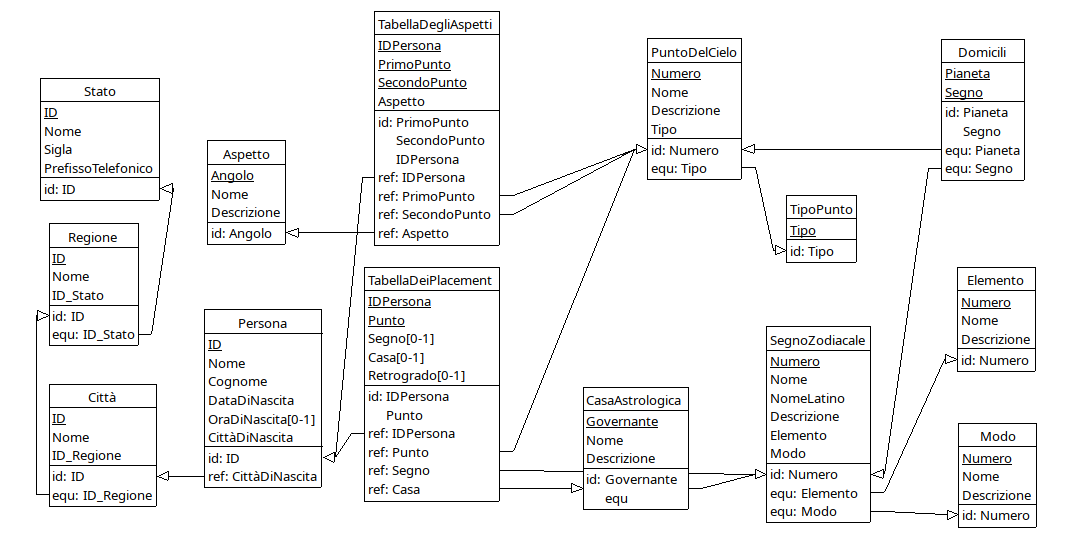
\includegraphics[width=\textwidth,height=\textheight,keepaspectratio]{img/finalschemelogic.png}
  \caption{Schema logico finale}
  \label{fig:finalschemelogic}
\end{sidewaysfigure}

\newpage

\section{Query SQL di Definizione}
CREATE TABLE Stato (\newline
\null\qquad ID int(11) NOT NULL AUTO\_INCREMENT PRIMARY KEY,\newline
\null\qquad Sigla varchar(3) NOT NULL,\newline
\null\qquad Nome varchar(150) NOT NULL,\newline
\null\qquad PrefissoTelefonico` int(11) NOT NULL,\newline
);\newline\newline
CREATE TABLE Regione (\newline
\null\qquad ID int(11) NOT NULL AUTO\_INCREMENT PRIMARY KEY,\newline
\null\qquad Nome varchar(255) NOT NULL,\newline
\null\qquad ID\_Stato int(11) NOT NULL DEFAULT '1',\newline
\null\qquad FOREIGN KEY (`ID\_Stato`) REFERENCES `Stato` (`ID`) \newline
\null\qquad ON DELETE CASCADE\newline
\null\qquad ON UPDATE CASCADE\newline
);\newline\newline
CREATE TABLE Citta (\newline
\null\qquad ID int(11) unsigned NOT NULL AUTO\_INCREMENT PRIMARY KEY,\newline
\null\qquad Nome varchar(30) NOT NULL,\newline
\null\qquad ID\_Regione int(11) NOT NULL,\newline
\null\qquad UNIQUE KEY `ID` (`ID`),\newline
\null\qquad FOREIGN KEY (`ID\_Regione`) REFERENCES `Regione` (`ID`) \newline
\null\qquad ON DELETE CASCADE\newline
\null\qquad ON UPDATE CASCADE\newline
);\newline\newline
CREATE TABLE Modo(\newline
\null\qquad Numero INT PRIMARY KEY,\newline
\null\qquad Nome VARCHAR(10) NOT NULL,\newline
\null\qquad Descrizione VARCHAR(200) NOT NULL\newline
);\newline\newline
CREATE TABLE Elemento(\newline
\null\qquad Numero INT PRIMARY KEY,\newline
\null\qquad Nome VARCHAR(5) NOT NULL,\newline
\null\qquad Descrizione VARCHAR(200) NOT NULL\newline
);\newline\newline
CREATE TABLE SegnoZodiacale(\newline
\null\qquad Numero INT PRIMARY KEY,\newline
\null\qquad Nome VARCHAR(15) NOT NULL,\newline
\null\qquad NomeLatino VARCHAR(15) NOT NULL,\newline
\null\qquad Descrizione VARCHAR(200) NOT NULL,\newline
\null\qquad Elemento INT NOT NULL,\newline
\null\qquad Modo INT NOT NULL,\newline
\null\qquad FOREIGN KEY(Elemento) REFERENCES Elemento(Numero)\newline
\null\qquad ON DELETE NO ACTION\newline
\null\qquad ON UPDATE CASCADE,\newline
\null\qquad FOREIGN KEY(Modo) REFERENCES Modo(Numero)\newline
\null\qquad ON DELETE NO ACTION\newline
\null\qquad ON UPDATE CASCADE\newline
);\newline\newline
CREATE TABLE CasaAstrologica(\newline
\null\qquad Governante INT PRIMARY KEY,\newline
\null\qquad Nome VARCHAR(30) NOT NULL,\newline
\null\qquad Descrizione VARCHAR(200) NOT NULL,\newline
\null\qquad FOREIGN KEY(Governante) REFERENCES SegnoZodiacale(Numero)\newline
\null\qquad ON DELETE NO ACTION\newline
\null\qquad ON UPDATE CASCADE\newline
);\newline\newline
CREATE TABLE Aspetto(\newline
\null\qquad Angolo INT PRIMARY KEY,\newline
\null\qquad Nome VARCHAR(20) NOT NULL,\newline
\null\qquad Descrizione VARCHAR(200) NOT NULL\newline
);\newline\newline
CREATE TABLE TipoPunto(\newline
\null\qquad Tipo VARCHAR(20) NOT NULL PRIMARY KEY\newline
);\newline\newline
CREATE TABLE PuntoDelCielo(\newline
\null\qquad Numero INT PRIMARY KEY,\newline
\null\qquad Nome VARCHAR(20) NOT NULL,\newline
\null\qquad Descrizione VARCHAR(200) NOT NULL,\newline
\null\qquad Tipo VARCHAR(20) NOT NULL,\newline
\null\qquad FOREIGN KEY(Tipo) REFERENCES TipoPunto(Tipo)\newline
\null\qquad ON DELETE NO ACTION\newline
\null\qquad ON UPDATE CASCADE\newline
);\newline\newline
CREATE TABLE Domicilio(\newline
\null\qquad Segno INT NOT NULL,\newline
\null\qquad Punto INT NOT NULL,\newline
\null\qquad PRIMARY KEY(Segno, Punto),\newline
\null\qquad FOREIGN KEY(Segno) REFERENCES SegnoZodiacale(Numero)\newline
\null\qquad ON DELETE CASCADE\newline
\null\qquad ON UPDATE CASCADE,\newline
\null\qquad FOREIGN KEY(Punto) REFERENCES PuntoDelCielo(Numero)\newline
\null\qquad ON DELETE CASCADE\newline
\null\qquad ON UPDATE CASCADE\newline
);\newline\newline
CREATE TABLE Persona(\newline
\null\qquad ID INT PRIMARY KEY AUTO\_INCREMENT,\newline
\null\qquad Nome VARCHAR(20) NOT NULL,\newline
\null\qquad Cognome VARCHAR(20) NOT NULL,\newline
\null\qquad DataDiNascita DATE NOT NULL,\newline
\null\qquad OraDiNascita TIME,\newline
\null\qquad CittaDiNascita INT(11),\newline
\null\qquad FOREIGN KEY(CittaDiNascita) REFERENCES Citta(ID)\newline
\null\qquad ON DELETE SET NULL\newline
\null\qquad ON UPDATE CASCADE\newline
);\newline\newline
CREATE TABLE TabellaDeiPlacement(\newline
\null\qquad IDPersona INT NOT NULL,\newline
\null\qquad Punto INT NOT NULL,\newline
\null\qquad Segno INT,\newline
\null\qquad Casa INT,\newline
\null\qquad Retrogrado BIT,\newline
\null\qquad PRIMARY KEY(IDPersona, Punto),\newline
\null\qquad FOREIGN KEY(IDPersona) REFERENCES Persona(ID)\newline
\null\qquad ON DELETE CASCADE\newline
\null\qquad ON UPDATE CASCADE,\newline
\null\qquad FOREIGN KEY(Punto) REFERENCES PuntoDelCielo(Numero)\newline
\null\qquad ON DELETE NO ACTION\newline
\null\qquad ON UPDATE CASCADE,\newline
\null\qquad FOREIGN KEY(Segno) REFERENCES SegnoZodiacale(Numero)\newline
\null\qquad ON DELETE NO ACTION\newline
\null\qquad ON UPDATE CASCADE,\newline
\null\qquad FOREIGN KEY(Casa) REFERENCES CasaAstrologica(Governante)\newline
\null\qquad ON DELETE NO ACTION\newline
\null\qquad ON UPDATE CASCADE\newline
);\newline\newline
CREATE TABLE TabellaDegliAspetti(\newline
\null\qquad IDPersona INT NOT NULL,\newline
\null\qquad PrimoPunto INT NOT NULL,\newline
\null\qquad SecondoPunto INT NOT NULL,\newline
\null\qquad Aspetto INT NOT NULL,\newline
\null\qquad PRIMARY KEY(IDPersona, PrimoPunto, SecondoPunto),\newline
\null\qquad FOREIGN KEY(IDPersona) REFERENCES Persona(ID)\newline
\null\qquad ON DELETE CASCADE\newline
\null\qquad ON UPDATE CASCADE,\newline
\null\qquad FOREIGN KEY(PrimoPunto) REFERENCES PuntoDelCielo(Numero)\newline
\null\qquad ON DELETE NO ACTION\newline
\null\qquad ON UPDATE CASCADE,\newline
\null\qquad FOREIGN KEY(SecondoPunto) REFERENCES PuntoDelCielo(Numero)\newline
\null\qquad ON DELETE NO ACTION\newline
\null\qquad ON UPDATE CASCADE,\newline
\null\qquad FOREIGN KEY(Aspetto) REFERENCES Aspetto(Angolo)\newline
\null\qquad ON DELETE NO ACTION\newline
\null\qquad ON UPDATE CASCADE\newline
);\newline

\section{Query SQL di Manipolazione}
Non verranno riportate le query banali, come quelle di inserimento o cancellazione di Persone, Placement e Aspetti. In riferimento alla sezione \ref{sec:opprinc}, le query per ricavare i dettagli astrologici di una persona sono le seguenti:\newline\newline\newline
\textbf{Ricavare il pianeta di domicilio del Segno Solare}\newline
SELECT p.`Nome` FROM `PuntoDelCielo` p JOIN `Domicilio` d ON p.`Numero` = d.`Punto` WHERE d.`Segno` =
(SELECT t.`Segno` FROM `TabellaDeiPlacement` t WHERE t.`IDPersona`=\textit{ID} AND t.`Punto`=1);\newline\newline
\textbf{Ricavare i pianeti in domicilio}\newline
SELECT p.`Nome` FROM `TabellaDeiPlacement` t JOIN `Domicilio` d \newline
ON t.`Segno` = d.`Segno` AND (t.`Punto` = d.`Punto`) \newline
JOIN `PuntoDelCielo` p ON t.`Punto` = p.`Numero` WHERE t.`IDPersona`=\textit{ID};\newline\newline
\textbf{Ricavare il numero di elementi tra i Placement di una persona:}\newline
SELECT COUNT(CASE WHEN s.`Elemento` = 1 THEN 1 ELSE NULL END) as Fuoco,
       COUNT(CASE WHEN s.`Elemento` = 2 THEN 1 ELSE NULL END) as Terra,
       COUNT(CASE WHEN s.`Elemento` = 3 THEN 1 ELSE NULL END) as Aria,
       COUNT(CASE WHEN s.`Elemento` = 4 THEN 1 ELSE NULL END) as Acqua
FROM `TabellaDeiPlacement` t JOIN `SegnoZodiacale` s ON t.`Segno`= s.`Numero` WHERE t.`IDPersona`=\textit{ID};\newline\newline
\textbf{Ricavare il numero di modi tra i Placement di una persona:}\newline
SELECT COUNT(CASE WHEN s.`Modo` = 1 THEN 1 ELSE NULL END) as Cardinale,
       COUNT(CASE WHEN s.`Modo` = 2 THEN 1 ELSE NULL END) as Fisso,
       COUNT(CASE WHEN s.`Modo` = 3 THEN 1 ELSE NULL END) as Mutevole
FROM `TabellaDeiPlacement` t JOIN `SegnoZodiacale` s ON t.`Segno`= s.`Numero` WHERE t.`IDPersona`=\textit{ID};\newline\newline
\textbf{Ricavare la casa piú popolata:}\newline
SELECT t.`Casa` FROM `TabellaDeiPlacement` t WHERE t.`IDPersona`=\textit{ID} GROUP BY (t.`Casa`) ORDER BY COUNT(*) DESC LIMIT 1;\newline\newline
\textbf{Ricavare la firma zodiacale:}\newline
SELECT s.`Nome` FROM `SegnoZodiacale` s JOIN `Modo` m ON s.`Modo`=m.`Numero` JOIN `Elemento` e ON s.`Elemento`= e.`Numero` WHERE m.`Nome`= \newline\newline
(SELECT m.`Nome` FROM `TabellaDeiPlacement` t JOIN `SegnoZodiacale` s ON t.`Segno`= s.`Numero`  JOIN `Modo` m ON s.Modo=m.Numero WHERE t.`Punto` <=10 AND t.`IDPersona`=\textit{ID} GROUP BY(m.`Nome`) ORDER BY COUNT(m.`Nome`) DESC LIMIT 1) \newline\newline
AND e.`Nome` =
\newline\newline
(SELECT e.`Nome` FROM `TabellaDeiPlacement` t JOIN `SegnoZodiacale` s ON t.`Segno`= s.`Numero`  JOIN `Elemento` e ON s.Elemento=e.Numero WHERE t.`Punto` <=10 AND t.`IDPersona`=\textit{ID} GROUP BY(e.`Nome`) ORDER BY COUNT(e.`Nome`) DESC LIMIT 1);
